
\section{Software}
Die Software gliedert sich in einen Teil für den Sensorprint auf dem Modul und einen Teil für den Meldeprint beim Gleichrichter. Der Teil für den Sensorprint muss unabhängig und wartungsfrei ablaufen können, wohingegen der Teil des Meldeprints in Interaktion mit dem Benutzer steht. Der Meldeprint bildet den wichtigsten Teil des Bindeglieds zwischen Benutzer und Hardware. Damit er die einzelnen Module identifizieren kann wird bei der Installation dem Sensorprints eine Identifikationsnummer gegeben. Zudem muss der Benutzer im Interface des Meldeprints die Anzahl Module angeben.
Die Gemessenen Spannungswerte der Module werden via Powerline an den Meldeprint gesendet. Es sollen keine extra Datenkabel verwendet werden. Diese Daten müssen in der Meldezentrale auf dem Meldeprint verarbeitet werden. Eine allfällige Abweichung des Spannungswertes bei einem oder mehreren Modulen sollen erkannt und identifiziert werden. Worin genau diese Abweichung besteht, wird später erläutert. Nach der Identifikation muss ein solcher Fehler gemeldet werden. Die Kommunikation zwischen Hardware und Software basiert auf SPI. Das Endprodukt setzt sich aus Melde- und Sensorprint zusammen. In dieser Unterteilung werden in den nächsten Kapiteln alle Softwarekomponenten beschrieben.
\newpage
\subsection{Sensorprint}
Der Sensorprint übernimmt die Spannungsmessung und sendet diese mit der Identifikationsnummer via Powerline an den Meldeprint. Die Kopplung in die Powerline gelingt mit einem Ferritkern. In den folgenden Kapiteln wird die Software weiter unterteilt und jeder Bereich einzeln erläutert.
\subsubsection{Aufbau und Abläufe}
Der Aufbau der Software auf der Sensorplatine basiert auf zwei verschiedenen Kommunikationsprotokollen. Zwischen dem ADC und dem Mikrocontroller via SPI und dem Mikrocontroller und dem Tranceiver via UART. In der Abbildung \ref{DiagrammSP} ist der Ablauf der Software dargestellt.

\begin{figure}[htb]
\centering
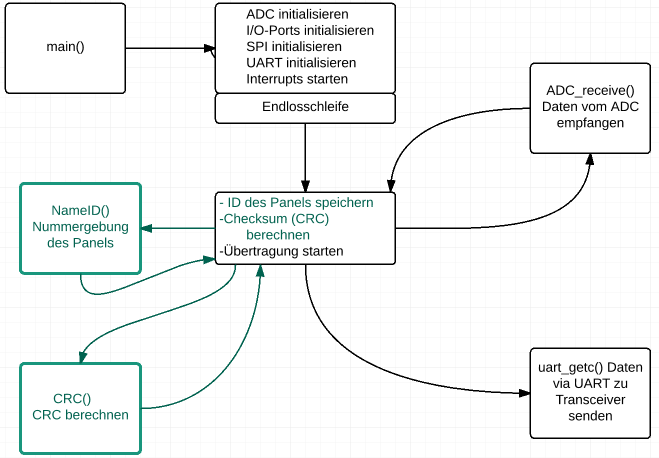
\includegraphics[width=0.8\textwidth]{sections/data/Sensorplatine}
\caption{Softwarekonzept der Sensorplatine}
\label{DiagrammSP}
\end{figure}

In der vorhergehenden Abbildung \ref{DiagrammSP} ist der Zusammenhang der einzelnen Teilprogramme ersichtlich. Aus dem $main()$ werden via der Endlosschlaufe die Unterprogramme, $ADC$\_$receive()$,$uart$\_$getc()$und zukünftig ebenfalls $CRC()$ und $NameID()$ aufgerufen. Die grünen Teile werden in Zukunft realisiert.\\

\paragraph{Inbetriebnahme}\\
Die Identifikationsnummer kann über das Einlesen der Dip-Schalter gespeichert bzw. definiert werden. Dies muss vom Benutzer eindeutig und selbständig eingestellt werden. Es ist wichtig, dass diese Identifikationsnummer eindeutig und einzigartig im gesamten String ist. Der Plan ist, dass man via USB dem Panel zusätzlich ein Name gibt, um die Identifikation der einzelnen Panel zu vereinfachen. 

\subsubsection{Spannungsmessung}
%wieso-was-wie-unter welchen Bedingungen
Die Kommunikation zwischen ADC und Mikrocontroller basiert auf dem Master-Salve-Prinzip. 
Als Basis für die Spannungsmessung soll zukünftig ein Referenzwert dienen. Der empfangene Wert soll durch Berechnung der Abweichung zu diesem Referenzwert dem Spannnungswert zugeteilt werden. Der Plan ist, dass die empfangenen Werte vom ADC vom Mikrocontroller in einem bestimmten Zeitraum gespeichert gespeichert werden und der Mittelwert weiter an den Transceiver geleitet wird.

\subsubsection{Transceiver-Ansteuerung}
%wieso-was-wie-unter welchen Bedingungen
Die Kommunikation zwischen dem Mikrocontroller und dem Tranceiver funktioniert über UART. 
Der Mittelwert der Spannungsmessung soll an den Transceiver weitergegeben werden. Der Plan ist, dass neben dem Spannungswert die mit dem Schaltern eingestellte Identifikationsnummer und eine Checksumme übergeben wird. Die Prüfsumme soll mit dem zyklische Redundanzprüfung (Cyclic redundancy check = CRC)  erstellt werden. Die Prüfsumme ist sehr wichtig, da die Kommunikation über die Powerline unidirektional sein soll und  mit Hilfe einer Prüfsumme Fehler, welche durch Kollisionen oder äussere Einflüsse entstehen, detektiert werden können.

\subsubsection{Kollisionsprävention}
















